\section{Kruskal-Wallis Test}
\subsection{Background}
\subsubsection{The One-Way Layout}
One-way, also known as single-factor, means that there is only one treatment among the groups in data. 

Denote the data consist of $N=\sum_{j=1}^{I} n_i$ observations, with $n_i$ observations from the $i$th treatment, $i=1, \dots, I$.

\begin{figure}[H]
	\centering
	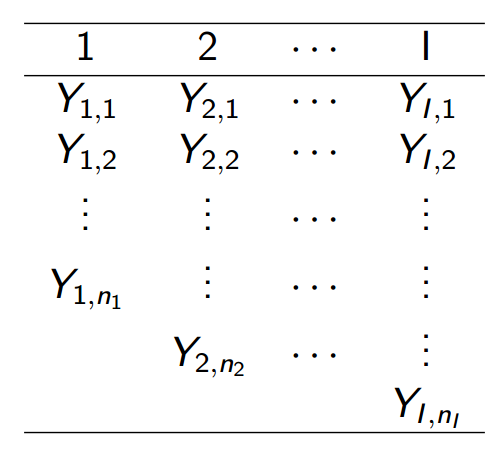
\includegraphics[width=0.3\linewidth]{fig/data}
	\caption{Data}
	\label{fig:data}
\end{figure}

Note that each group can have different number of observations.
\subsubsection{One-Way ANOVA}
In statistics, one-way analysis of variance is a technique that can be used to compare means(location) of two \textbf{or more samples}. The primary interest consist in comparing the location of three of more samples.

\begin{itemize}
	\item Null Hypothesis: the sample data are supposed to come from the same population.
	\item Alternative Hypothesis: the sample data are supposed to come from different populations.
\end{itemize}

Recall in ANOVA, the variability of data is broken down into two components:
\begin{itemize}
	\item Sum of squares of the columns: between groups variability, due to the different locations of the populations.
	\item Sum of squares of the error: within groups variability, due to the variability in the population.
\end{itemize}

\begin{figure}[H]
	\centering
	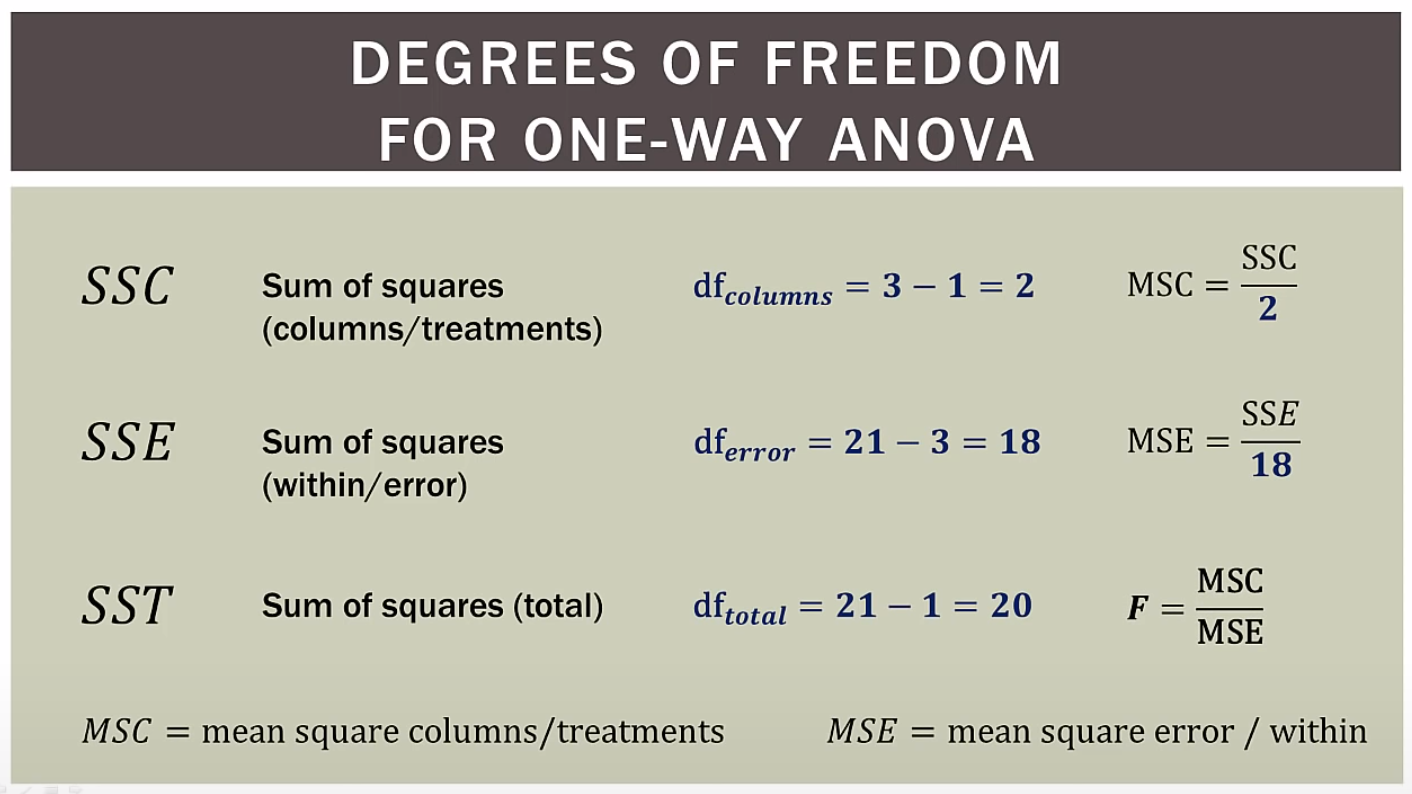
\includegraphics[width=0.7\linewidth]{fig/anova}
	\caption{Analysis of Variance}
	\label{fig:anova}
\end{figure}

$F$-ratio is the test statistic for the hypothesis test.

\subsection{Assumption}
\begin{itemize}
	\item The random variables are all mutually independent.
	\item Random variables in the same group follow the same continuous distribution $F_i$, $i=1, \dots, I$.
	\item $F_i(t) = F(t-\tau_i)$, $-\infty < t < \infty$.
	\begin{itemize}
		\item $F$ is a continuous distribution function with unknown median $\theta$;
		\item $\tau_i$ is the unknown treatment effect for the $i$-th population.
		\item No difference in scale parameters (variability).
	\end{itemize}
\end{itemize}

We can set up the model of each observation based on the assumptions.
\[Y_{ik} = \theta + \tau_i + \epsilon_{ik}\]

\begin{itemize}
	\item $i = 1, \dots, I, k = 1, \dots, n_i$.
	\item $\theta$: overall median.
	\item $\tau_i$: the $i$-th treatment effect.
	\item $\epsilon_{ik}$: random error. iid from a continuous distribution with median 0.
\end{itemize}

\subsection{Hypothesis}
\begin{itemize}
	\item $H_0$: $\tau_1 = \cdots = \tau_I$, which means that $F_1 = \cdots = F_I = F$.
	\item $H_1$: $\tau_1 \dots \tau_I$ are not all equal.
\end{itemize}
\subsubsection{Rank}
Combine all $N$ observations from the $I$ groups and order them from least to greatest.
\begin{figure}[H]
	\centering
	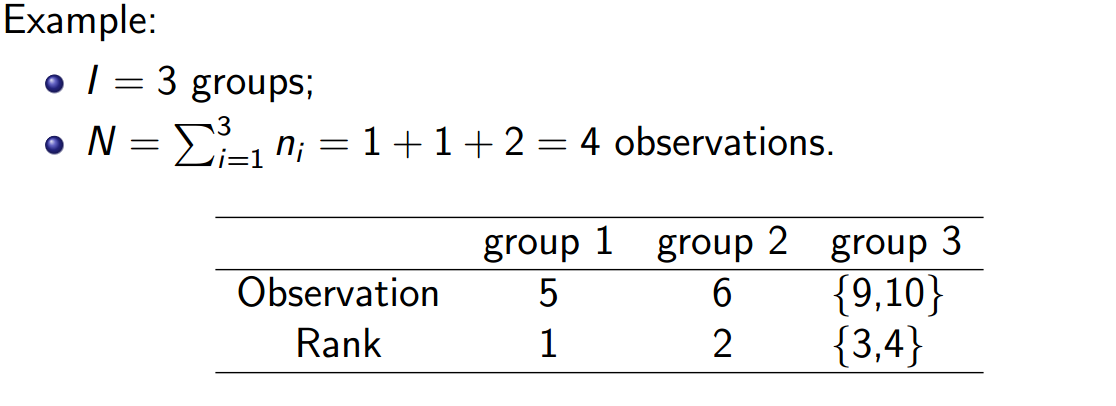
\includegraphics[width=0.7\linewidth]{fig/rank}
	\caption{Example: Rank}
	\label{fig:rank}
\end{figure}

\subsubsection{Test Statistic}

Let $r_{ik}$ denotes the rank of $Y_{ik}$ in this joint ranking. The average rank assigned in the joint ranking is 
\[\frac{1}{N}\sum_{i = 1}^{I} \sum_{k=1}^{n_i} r_{ik} = \frac{N(N+1)}{2N} = \frac{N + 1}{2}\]

Let $R_i = \sum_{k=1}^{n_i} r_{ik}$, which is the sum of the joint ranks received by the observations in the $i$-th group.

Let $\bar{R}_i = R_i / n_i$, $i = 1, \dots, I$, which is the average rank received by observations in the $i$-th group.

The Kruskal-Wallis statistic $H$ is then given by
\begin{align*}
	H 
	&= \frac{12}{N(N+1)} \sum_{i=1}^{I} n_i (\bar{R}_i - \frac{N+1}{2})^2\\
	&= (\frac{12}{N(N+1)} \sum_{i=1}^{I} \frac{R_i^2}{n_i}) - 3(N+1).
\end{align*}

Reject $H_0$ if $H \ge h_\alpha$, the upper $\alpha$ percentile for the null distribution of $H$.

Under the Null Hypothesis, 
\begin{itemize}
	\item $\E r_{ik} = \frac{N+1}{2}$
	\item $\E \bar{R}_i = \frac{1}{n_i} \sum_{k=1}^{n_i} r_{ik} = \frac{1}{n_i} n_i \E r_{ik} = \frac{N + 1}{2}$.
\end{itemize}


Intuitively, we expect the $\bar{R}_i$'s to be close to $\frac{N+1}{2}$ when $H_0$ is true. So that small values of $H$ represent agreement with $H_0$. 

Otherwise, when the $\tau$'s are not all equal, we would expect a portion of the associated treatment average ranks to differ from their common average, $(N+1)/2$, with some tending to be larger and some smaller. Hence, the net result $n_i(\bar{R}_i - \frac{N+1}{2})^2$ would lead to a large value of $H$. This suggests rejecting $H_0$ in favor of $H_1$ for large values of $H$.

\begin{figure}[H]
	\centering
	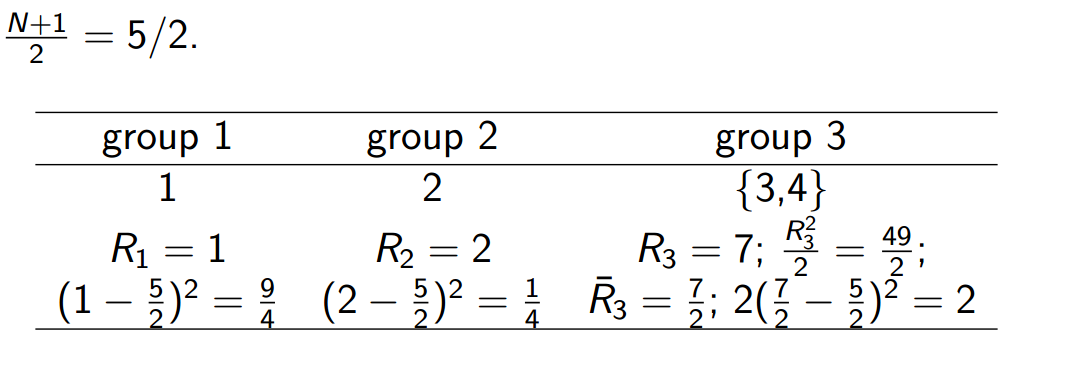
\includegraphics[width=0.7\linewidth]{fig/kruskal-wallis}
	\caption{Example: Kruskal-Wallis Test}
	\label{fig:kruskal-wallis}
\end{figure}

\subsection{Extensions}
Recall that the alternative hypothesis of Kruskal-Wallis Test is that $\tau_i$'s are not equal. Now we introduce two more test for stronger alternative hypothesis.

\subsubsection{Jonckheere-Terpstra Test}
In many practical settings, the treatments are such that the
appropriate alternatives to no differences in treatment effects
(H0) are those of increasing (or decreasing) treatment effects
according to some natural labeling for the treatments.

Examples of such settings include ``treatments'' corresponding to
degrees of knowledge of performance, quality or quantity of
materials, severity of disease, amount of practice, drug dosage
levels, intensity of a stimulus, and temperature.

The Kruskal-Wallis test does not utilize any such partial prior
information regarding a postulated alternative ordering.

The alternative hypothesis for Jonckheere-Terpstra Test is that
\[H_1: \tau_1 \le \tau_2 \le \cdots \le \tau_I\]
, with at least one strict inequality.

\subsubsection{Mack-Wolfe Test}
The alternative hypothesis for Mack-Wolfe Test is that
\[H_1: \tau_1 \le \cdots \le \tau_p \ge \tau_{p+1} \ge \cdots \tau_I\]
, with at least one strict inequality.

The distribution of $\tau_i$'s are in the shape of umbrella. But this test rarely used nowdays.